% Options for packages loaded elsewhere
\PassOptionsToPackage{unicode}{hyperref}
\PassOptionsToPackage{hyphens}{url}
\PassOptionsToPackage{dvipsnames,svgnames*,x11names*}{xcolor}
%
\documentclass[
  11pt,
]{article}
\usepackage{amsmath,amssymb}
\usepackage{lmodern}
\usepackage{ifxetex,ifluatex}
\ifnum 0\ifxetex 1\fi\ifluatex 1\fi=0 % if pdftex
  \usepackage[T1]{fontenc}
  \usepackage[utf8]{inputenc}
  \usepackage{textcomp} % provide euro and other symbols
\else % if luatex or xetex
  \usepackage{unicode-math}
  \defaultfontfeatures{Scale=MatchLowercase}
  \defaultfontfeatures[\rmfamily]{Ligatures=TeX,Scale=1}
\fi
% Use upquote if available, for straight quotes in verbatim environments
\IfFileExists{upquote.sty}{\usepackage{upquote}}{}
\IfFileExists{microtype.sty}{% use microtype if available
  \usepackage[]{microtype}
  \UseMicrotypeSet[protrusion]{basicmath} % disable protrusion for tt fonts
}{}
\makeatletter
\@ifundefined{KOMAClassName}{% if non-KOMA class
  \IfFileExists{parskip.sty}{%
    \usepackage{parskip}
  }{% else
    \setlength{\parindent}{0pt}
    \setlength{\parskip}{6pt plus 2pt minus 1pt}}
}{% if KOMA class
  \KOMAoptions{parskip=half}}
\makeatother
\usepackage{xcolor}
\IfFileExists{xurl.sty}{\usepackage{xurl}}{} % add URL line breaks if available
\IfFileExists{bookmark.sty}{\usepackage{bookmark}}{\usepackage{hyperref}}
\hypersetup{
  colorlinks=true,
  linkcolor=Maroon,
  filecolor=Maroon,
  citecolor=Blue,
  urlcolor=blue,
  pdfcreator={LaTeX via pandoc}}
\urlstyle{same} % disable monospaced font for URLs
\usepackage[margin=1in]{geometry}
\usepackage{graphicx}
\makeatletter
\def\maxwidth{\ifdim\Gin@nat@width>\linewidth\linewidth\else\Gin@nat@width\fi}
\def\maxheight{\ifdim\Gin@nat@height>\textheight\textheight\else\Gin@nat@height\fi}
\makeatother
% Scale images if necessary, so that they will not overflow the page
% margins by default, and it is still possible to overwrite the defaults
% using explicit options in \includegraphics[width, height, ...]{}
\setkeys{Gin}{width=\maxwidth,height=\maxheight,keepaspectratio}
% Set default figure placement to htbp
\makeatletter
\def\fps@figure{htbp}
\makeatother
\setlength{\emergencystretch}{3em} % prevent overfull lines
\providecommand{\tightlist}{%
  \setlength{\itemsep}{0pt}\setlength{\parskip}{0pt}}
\setcounter{secnumdepth}{-\maxdimen} % remove section numbering
\usepackage{setspace}
\usepackage{float}
\usepackage{mathtools}
\usepackage{natbib}
\usepackage[linesnumbered,ruled,vlined]{algorithm2e}
\setcitestyle{numbers,square,comma}
\usepackage{verbatim}
\usepackage{amsthm}
\usepackage{comment}
\ifluatex
  \usepackage{selnolig}  % disable illegal ligatures
\fi
\usepackage[]{natbib}
\bibliographystyle{plainnat}

\title{Semi-Parametric Manifold Clustering}
\author{}
\date{\vspace{-2.5em}}

\begin{document}
\maketitle

\newcommand{\diag}{\mathrm{diag}}
\newcommand{\tr}{\mathrm{Tr}}
\newcommand{\blockdiag}{\mathrm{blockdiag}}
\newcommand{\indep}{\stackrel{\mathrm{ind}}{\sim}}
\newcommand{\iid}{\stackrel{\mathrm{iid}}{\sim}}
\newcommand{\Bernoulli}{\mathrm{Bernoulli}}
\newcommand{\Betadist}{\mathrm{Beta}}
\newcommand{\Uniform}{\mathrm{Uniform}}
\newcommand{\BG}{\mathrm{BernoulliGraph}}
\newcommand{\Categorical}{\mathrm{Categorical}}
\newcommand{\Multinomial}{\mathrm{Multinomial}}
\newcommand{\RDPG}{\mathrm{RDPG}}
\newcommand{\GRDPG}{\mathrm{GRDPG}}
\newtheorem{definition}{Definition}
\newtheorem{theorem}{Theorem}
\newtheorem{lemma}{Lemma}
\theoremstyle{remark}
\newtheorem*{remark}{Remark}
\theoremstyle{example}
\newtheorem{example}{Example}
\newcommand{\dd}{\mathrm{d}}
\newcommand{\as}{\stackrel{\mathrm{a.s.}}{\to}}
\newcommand{\ind}{\stackrel{\mathrm{ind}}{\sim}}

\hypertarget{estimating-polynomial-curves}{%
\section{Estimating Polynomial
Curves}\label{estimating-polynomial-curves}}

\hypertarget{problem-setup}{%
\subsection{Problem Setup}\label{problem-setup}}

Let:

\begin{itemize}
\tightlist
\item
  \(T_1, ..., T_n \stackrel{\mathrm{iid}}{\sim}F\) with support
  \([0, 1]\).
\item
  \(g(\cdot, \theta) : [0, 1] \mapsto \mathcal{X} \subset \mathbb{R}^d\).
\item
  \(X_1, ..., X_n = g(T_1), ..., g(T_n)\)
\end{itemize}

Assuming some parametric form of \(g\) with parameters \(\theta\), we
want to find \(\hat{\theta}\), some ``reasonable'' estimate for
\(\theta\). We observe \(X_i\) but not \(T_i\).

For now, we limit \(d = 2\) and \(g\) to quadratic functions.

\begin{example}

Let $g(t) = (t^2, 2 t (1 - t) ) = (0 + 0 t + t^2, 0 + 2 t - 2 t^2)$. 
(This is the first two dimensions of the Hardy-Weinberg curve). 
Then $\theta = (0, 0, 1, 0, 2, -2)$.


\begin{center}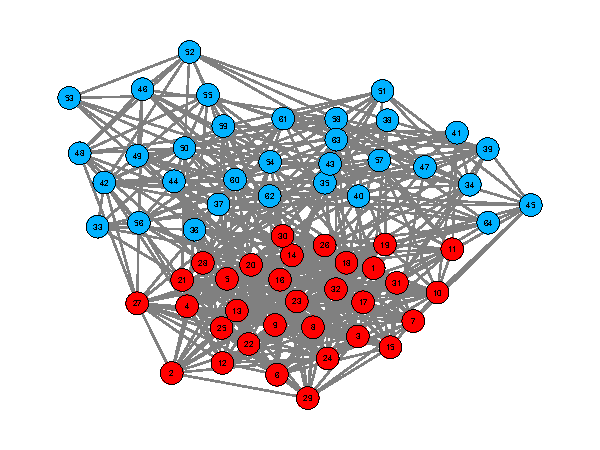
\includegraphics{curve-fitting-scratch_files/figure-latex/unnamed-chunk-2-1} \end{center}

\end{example}

If we observe the \(T_i\)'s, then we can use a standard polynomial
regression method to obtain \(\hat{\theta}\). Since we do not observe
them, the proposed iterative method is as follows:

\begin{enumerate}
\def\labelenumi{\arabic{enumi}.}
\tightlist
\item
  Initialize \(\hat{\theta}^{(0)}\) (e.g., randomly).
\item
  Estimate each \(\hat{t}_i^{(s)}\) by minimizing
  \(L(t_i, \hat{\theta}^{(s)} | x_i) = L_i = \|x_i - g(t_i | \hat{\theta}^{(s)})\|^2\).
\item
  Compute each
  \(\hat{x}_i^{(s)} = g(\hat{t}_i^{(s)} | \hat{\theta}^{(s)})\)
\item
  Estimate \(\hat{\theta}^{(s+1)}\) by minimizing
  \(L(\{\hat{t}_i^{(s)}\}, \theta | X) = \sum_i \|x_i - g(\hat{t}_i^{(s)} | \theta)\|^2\).
\item
  Repeat steps 2-4 until convergence.
\end{enumerate}

If we restrict \(g\) to be polynomials, then steps (2) and (4) have
closed-form solutions. Alternatively, we can estimate \(g\) using more
general forms, e.g., splines, which may require approximation.

\begin{example}

Write $g(t | \theta) = (g_1(t | \theta_1), ..., g_d(t | \theta_d))$ where $g_r(t | \theta_r)$ is the component of $g$ in the $r^{th}$ dimension and $\theta_r$ is the vector of parameters for the $r^{th}$ dimension. If $g_r$ are polynomials of degree $p$, then each $\theta_r$ contains up to $p + 1$ entries. 

Given the observed points $x_1, ..., x_n \in \mathbb{R}^d$ and their corresponding index points $t_1, ..., t_n \in \mathbb{R}$, we can find each $\hat{\theta}_r$ individually by $\hat{\theta}_r = A^{-1} b$ where $b \in \mathbb{R}^{p+1}$ and $b_k = \sum_i x_i t_i^k$ and $A \in \mathbb{R}^{(p+1) \times (p+1)}$ and $A_{kl} = \sum_i t^{(k-1) (l-1)}$.

On the other hand, if we have parameters $\theta$ but not the index points $t_i$, we can minimize each $t_i$ individually by finding the roots of a $p+1$ polynomial with coefficients that depend on $x_1, ..., x_n$ and $\theta$. 

In the following plot, we drew $n = 200$ points from the 2D H-W curve with $T_1, ..., T_n \stackrel{\mathrm{iid}}{\sim}Uniform(0, 1)$. 
The red line is the curve that was fit using the above method. 

\end{example}

\begin{center}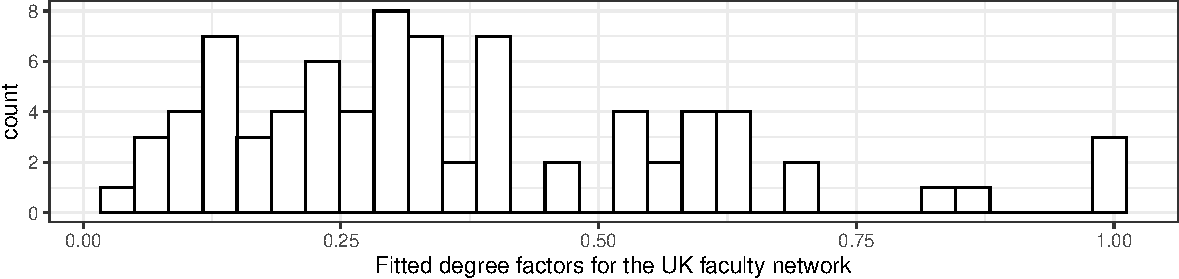
\includegraphics{curve-fitting-scratch_files/figure-latex/unnamed-chunk-3-1} \end{center}

Note: the parameterization of the curve is not unique.

\hypertarget{estimation-with-noise}{%
\section{Estimation with Noise}\label{estimation-with-noise}}

\begin{example}

In the next example, we draw $A \sim \mathrm{RDPG}(X)$ using the same H-W curve and sample size as above and estimate the true latent positions (up to rotation). 

\end{example}

\begin{center}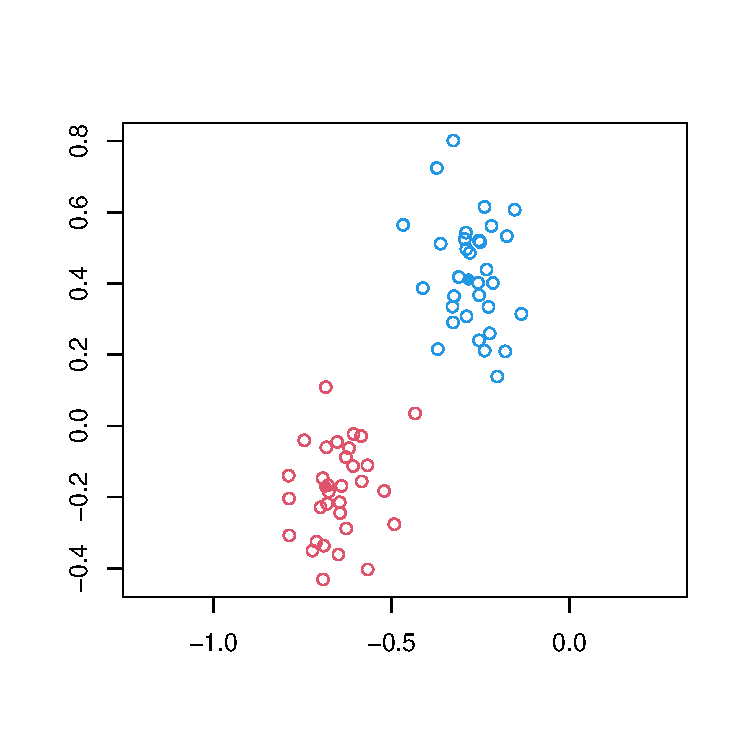
\includegraphics{curve-fitting-scratch_files/figure-latex/unnamed-chunk-5-1} \end{center}

A modification to this that is possibly more robust is to use Bezier
curves for \(g\). This is the same functional form as the polynomial
curves used before, but with orthogonal bases:

\[g(t | p) = \sum_{r = 0}^{R} p_r \binom{R}{r} (1 - t)^{R - r} t^r\]

where \(R\) is the order of the Bezier curve, each \(p_s\) is a vector
of length \(d\), and, as before, \(g : [0, 1] \mapsto \mathbb{R}^d\).
Thus, if we fit each \(p_r\), then the procedure is the same as before.

The least squares estimate for \(p \in \mathbb{R}^{R \times d}\) is

\[\hat{p} = (T^\top T)^{-1} T^\top X\]

where
\(T = \begin{bmatrix} t_{\cdot, 1} & \cdots & t_{\cdot, R} \end{bmatrix}\)
and each \(t_{ir} = \binom{R}{r} (1 - t_i)^{R - r} t_i^r\), and
\(X \in \mathbb{R}^{n \times d}\). The same procedure for estimating
\(t_1, ..., t_n\) can be applied here.

The parameterization for a given curve is not unique. In particular, the
above procedure will not necessarily provide
\(t_1, ..., t_n \in [0, 1]\). One possible remedy for this is to, after
estimating the \(t_i\)'s, normalize them to the unit interval. If we
assume \(t_1, ..., t_n \stackrel{\mathrm{iid}}{\sim}Uniform(a, b)\),
then the UMVUE are

\[\hat{a} = \frac{n t_{(1)} - t_{(n)}}{n - 1},
\hat{b} = \frac{n t_{(n)} - t_{(1)}}{n - 1}\]

which yields the normalization transformation
\(t \leftarrow (t - \hat{a}) / (\hat{b} - \hat{a})\).

Alternatively, we can force the \(t_i\)'s to be approxiately uniform on
the unit interval by the transformation \(t \leftarrow \hat{F}(t)\),
where \(\hat{F}\) is the empirical CDF of \(t_1, ..., t_n\).

For initialization, we can use a one-dimensional Isomap embedding to
estimate the \(t_i\)'s and use that to estimate \(\hat{p}\). Experiments
suggest that if the data are well-behaved (i.e., it looks like the curve
we are trying to fit), this results in much faster convergence.

\hypertarget{theoretical-framework}{%
\subsection{Theoretical Framework}\label{theoretical-framework}}

If we assume that the points are distributed as
\(X_i \stackrel{\mathrm{ind}}{\sim}\mathcal{N}(f(t_i | p), \Sigma(t_i | \phi))\),
then we can write the (incomplete) log likelihood as:

\[\ell(p, \phi) = -\frac{1}{2} \sum_i \log |\Sigma(t_i | \phi)| - \frac{1}{2} \sum_i (x_i - f(t_i | p))^\top (\Sigma(t_i | \phi))^{-1} (x_i - f(t_i | p))\]

In the case \(\Sigma(t_i | \phi) = \phi I\) and
\(f(t_i | p) = p^\top \tilde{t}_i\) where
\(\tilde{t}_i \in \mathbb{R}^{R+1}\) is the Bezier polynomial expansion
of order \(R\), then this becomes

\[\ell(p, \phi) = -\frac{n d}{2} \log \phi - \frac{1}{2 \phi} \|X - T p\|^2_F\]

Then given \(t_1, ..., t_n\), the MLE of \(p\) is again
\((T^\top T)^{-1} T^\top X\), and the MLE of \(\phi\) is just
\(\frac{1}{n d} \|X - T \hat{p}\|^2_F\). And given \(p\), we can
estimate each \(t_i\) in the same way as before to maximize \(\ell\)
(the variance is unnecessary here).

As noted before, the parameterization given by \(T\) and \(p\) is not
unique. We can arbitrarily scale the \(t_i\)'s and \(p\) to obtain the
same value of \(\ell\). Naively performing the proposed algorithm
sometimes results in estimates for \(p\) that diverge and estimates for
\(t_i\)'s that converge to a single value. To remedy this, we can either
scale the \(t_i\)'s as before, or we can scale \(p\) by forcing \(f\) to
be an arclength parameterization.

\begin{theorem}
Let $x_1, ..., x_n \stackrel{\mathrm{ind}}{\sim}\mathcal{N}(p^\top \tilde{t}_i, \phi I_d)$,
where each $x_i \in \mathbb{R}^d$, $\tilde{t}_i \in \mathbb{R}^{R+1}$ such that $\tilde{t}_{i,r} = \binom{R}{r} (1 - t_i)^{R-r} t_i^r$ for $i = 1, ..., n$ and $r = 0, ..., R$, 
and $p \in \mathbb{R}^{(R+1) \times d}$.

Then each iteration of the following decreases the negative log likelihood:

\begin{enumerate}
  \item $p \leftarrow (T^\top T)^{-1} T^\top X$, 
  where $T = \begin{bmatrix} \tilde{t}_1 & \cdots & \tilde{t}_n \end{bmatrix}^\top$ 
  and $X = \begin{bmatrix} x_1 & \cdots & x_n \end{bmatrix}^\top$.
  \item $t_i \leftarrow \arg\min_t \|x_i - p^\top \tilde{t}_i\|^2$,
  which can be solved by finding the roots of a polynomial of degree $2 R - 1$.
\end{enumerate}
\end{theorem}

\begin{proof}[Proof (sketch)]

For $\Sigma(t_i | \phi) = \phi I$, the negative log likelihood is, 
up to some additive and multiplicative constants:

$$l(p, \{t_i\}) = \|X - T p\|^2_F = X^\top X - 2 X^\top T p + p^\top T^\top T p$$

To find the minimizer $\hat{p}$ given $t_1, ..., t_n$:

$\nabla_p l = -2 T^\top X + 2 T^\top T p = 0$  
$\implies \hat{p} = (T^\top T)^{-1} T^\top X$

To find the minimizer $\hat{t}_i$ given $p$:

We can rewrite the negative log likelihood as 
$l(p, \{t_i\}) = \sum_i \|x_i - p^\top \tilde{t}_i\|^2$. 

Then each entry of $\nabla_{t} l$ depends only on $t_i$, so each $t_i$ can be optimized independently. 
Furthermore, each $\frac{\partial}{\partial t_i} \|x_i - p^\top \tilde{t}_i\|^2$ is a polynomial in $t_i$, so it can be minimized by simply finding the roots of the polynomial. 

Thus this algorithm is a coordinate descent algorithm, which reduces the objective function with each iteration. 
\end{proof}

\begin{theorem}

Let $A^{(n)} \sim \mathrm{RDPG}(F(p, \theta), n)$, and let $X^{(n)}$ be the ASE of $A^{(n)}$. 
Let $\hat{p}, \{\hat{t}_i\}$ be the global minimizer of $l$ given $X^{(n)}$. 
Then $l(\hat{p}, \{\hat{t}_i\}) \stackrel{a.s.}{\to} 0$. 

\end{theorem}

\hypertarget{covariance-structures}{%
\subsubsection{Covariance Structures}\label{covariance-structures}}

While the CLT property of the ASE allows us to approximate
\(x_i \sim \mathcal{N} (W f(t_i | p), W \Sigma(t_i | \phi) W^\top)\), it
is unclear what \(\Sigma(t_i | \phi)\) looks like, and we cannot in
general say \(\Sigma(t_i | \phi) = \phi I_d\).

\hypertarget{clustering}{%
\section{Clustering}\label{clustering}}

Next, suppose we have K curves parameterized by \(g^{(k)}\), with points
drawn along these curves. Then one possible clustering technique is as
follows:

\begin{enumerate}
\def\labelenumi{\arabic{enumi}.}
\tightlist
\item
  Assign an initial clustering (e.g., via spectral clustering).
\item
  Estimate the curve for each cluster (using the same curve-fitting
  procedure as before).
\item
  Reassign the clusters by proximity to each curve.
\item
  Repeat 2 and 3 until convergence.
\end{enumerate}

\begin{example}



We have two intersecting curves, $g_1(t) = \begin{bmatrix} t^2 & 2 t (1 - t) \end{bmatrix}^\top$ and $g_2(t) = \begin{bmatrix} 2 t (1 - t) & (1 - t) ^ 2 \end{bmatrix}^\top$. $n_1 = n_2 = 256$ points are drawn uniformly from each.


\begin{center}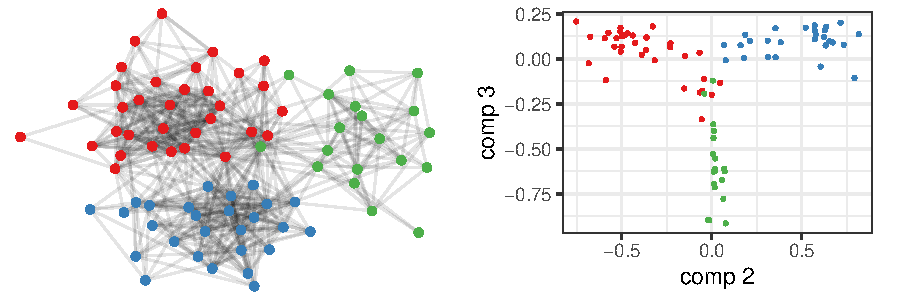
\includegraphics{curve-fitting-scratch_files/figure-latex/unnamed-chunk-7-1} \end{center}

We draw $A \sim \mathrm{RDPG}(X)$ and obtain the following ASE:


\begin{center}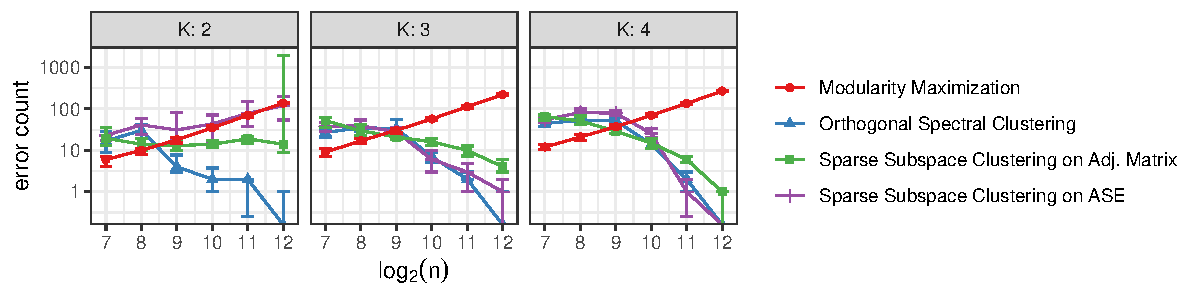
\includegraphics{curve-fitting-scratch_files/figure-latex/unnamed-chunk-8-1} \end{center}

Fitting two quadratic Bezier curves to these data yields a community detection error rate of 10\%. 
In the following plot, the points are labeled according to their estimated labels.


\begin{center}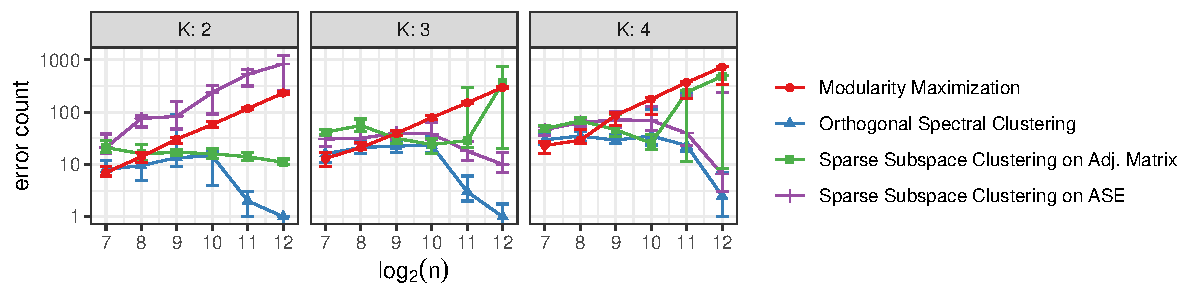
\includegraphics{curve-fitting-scratch_files/figure-latex/unnamed-chunk-9-1} \end{center}

\end{example}

The objective function that this method aims to minimize is:

\[\sum_{k=1}^K \sum_{i \in C_k} \|x_i - g_k(t_i | p_k)\|^2\]

Where \(g_k : [0, 1] \mapsto \mathbb{R}^d\) with parameters \(p_k\) is
the curve for community \(k\).

\textbf{TBD}: It can be shown that each iteration decreases the
objective unless we are at a stationary point.

\hypertarget{harry-potter-emnity-graph}{%
\subsection{Harry Potter Emnity Graph}\label{harry-potter-emnity-graph}}

\begin{example}
In this section, we analyze the Harry Potter emnity graph. 
Rubin-Delanchy et al. suggested applying the GRDPG ASE to this graph with $p = 1$ and $q = 1$, revealing a DCBM-like structure in the latent space. 
Passino and Heard instead fit Gaussian processes to the embedding. 
Here, we consider what happens when we apply the Bezier curve clustering method. 
\end{example}

\begin{center}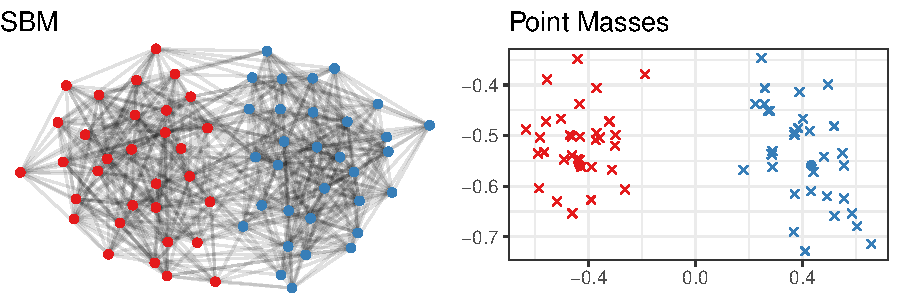
\includegraphics{curve-fitting-scratch_files/figure-latex/unnamed-chunk-11-1} \end{center}

  \bibliography{misc.bib}

\end{document}
